% vim: set spelllang=fr:

\setchapterpreamble[ur][\textwidth]{%
  \dictum[Bill Watterson, \textit{Calvin et Hobbes}]{%
    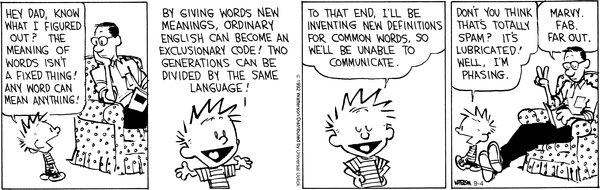
\includegraphics[width=\textwidth]{fig/calvin_meaning.png}}}

\chapter{Annotation en rôle sémantique en domaine spécifique}
\label{ch:domainsrl}

Là où le précédent chapitre présentait notre approche générique d'annotation en
rôles sémantiques fondée sur la connaissance, celui-là cherche à évaluer son
application en domaines spécifiques. À l'heure où les algorithmes supervisés
obtiennent d'excellentes performances sur un certain nombre de tâches quand des
données annotées pour le domaine considéré existent, l'adaptation au domaine
est un défi majeur en Traitement Automatique des Langues, et l'annotation en
rôles sémantiques sur de nouveaux domaines reste un problème ouvert.

Dans ce chapitre, nous n'utilisons pas le système du Chapitre~\ref{ch:srl} et
ne développons pas un système, mais nous évaluons la capacité de VerbNet et
\verbenet{} à traiter des corpus en domaines spécifiques.

La définition du terme 'domaine' reste assez vague dans le sens où il est
difficile de proposer une catégorisation de la connaissance en un ensemble de
domaines qui soit à la fois cohérente et efficace \citep{ma2012rethinking}. Il
est aussi difficile de séparer clairement le «~domaine général~» des domaines
spécifiques. Néanmoins, c'est un phénomène qui existe et qui est à considérer :
les modèles entraînés sur un corpus d'un domaine spécifique (la finance par
exemple) risque de produire des performances mauvaises si appliqués à d'autres
domaines (le football par exemple). C'est le cas par exemple de la
désambiguïsation de classe VerbNet au moment de passer du corpus PropBank à un
corpus du domaine biomédical \citep{abend2008supervised}.

Il est important aussi de différencier le genre et le domaine d'un texte. Le
corpus du Wall Street Journal traite du domaine de la finance dans un genre
journalistique. D'autres genres existent, par exemple les genre littéraires que
sont la fiction, la poésie, le théâtre, etc. Néanmoins, ces distinctions ne
nous concernent pas ici, et l'objectif affiché est de traiter aussi bien un
roman qu'une encyclopédie, un email bien écrit qu'un article de journal.  C'est
une simplification mais les difficultés que nous rencontrons avec les corpus
utilisés dépendent plutôt du domaine que du genre. En effet, nous supposons que
dans deux domaines différents plus que dans deux genres différents, les
changements vont résider dans les verbes utilisés, leur sens et la façon de les
utiliser. C'est ce que nous souhaitons prendre en compte ici.

\section{Corpus considérés}

Afin de s'assurer que notre travail reste valide en changeant de domaine, nous
considérons ici trois corpus présents dans des domaines différents.

\begin{itemize}

    \item le Kicktionary \citep{schmidt2006interfacing,schmidt2009kicktionary}
        rassemblant des dépêches de l'UEFA dans le domaine du football à propos
        de la Ligue Europa, de la Champions League et de la Coupe du Monde. Ce
        corpus est disponible en français, anglais et allemand.

    \item Le DiCoInfo est le corpus Informatique/Internet de l'OLST
        \citep{corpusolst} en anglais, français et espagnol.

    \item Le DiCoEnviro est le corpus Réchauffement climatique de l'OLST
        \citep{corpusolst} en anglais, français et espagnol.

\end{itemize}

Les deux intérêts majeurs communs à ces trois corpus sont :

\begin{enumerate}

    \item de s'inspirer plus ou moins librement de la méthodologie FrameNet, ce
        qui permet d'appliquer nos méthodes,

    \item d'être disponible à la fois en anglais et en français, ce qui permet
        de comparer VerbNet à \verbenet{},

    \item et d'être basés sur l'annotation dans un corpus d'un certain nombre
        de prédicats (ce n'est pas une annotation dite "full-text")

\end{enumerate}

Ce dernier point est plutôt un inconvénient : la manière la plus réaliste de
considérer un corpus d'entraînement est de réaliser une annotation dite
\textit{full-text} en annotant tous les prédicats rencontrés dans un texte
donné. Cependant, les contextes choisis l'ont été à chaque fois sur des
critères de diversité syntaxique
\citep{schmidt2006interfacing,lhomme2012adding}. Le postulat que nous faisons
dans ce travail est que notre méthode est moins affectée par ce problème qu'un
modèle statistique se basant exclusivement sur la distribution des différentes
constructions.

Les trois corpus ont étés découpés en deux parties de tailles égales : un
corpus d'entraînement et un corpus de test. Étant donné qu'il n'y a pas de
modèle à entraîner, ce corpus d'entraînement est simplement utilisé pour
comprendre les erreurs en l'analysant manuellement. Même si les trois corpus
contiennent des textes proches entre eux, ils sont issus de sources différentes
et ont étés écrits par des auteurs différents. Nous avons normalisé ces sources
(par exemple, les sources DEBIAN2 et DEBIAN3 dans le corpus Informatique \&
Internet de l'OLST ont manuellement été transformées verbs DEBIAN) et utilisons
cette information pour faire le découpage : une source spécifique ne peut être
présente que dans un ensemble. Le découpage résultant est disponible au format
JSON avec le code source associé à ce chapitre. Ce découpage ne nécessite pas
d'avoir normalisé les sources : chaque phrase est simplement associée à
l'ensemble de test ou l'ensemble d'entraînement.

\section{Mappings de rôles}

Ces trois corpus utilisent des rôles spécifiques. Les corpus DiCoInfo et
DiCoEnviro utilisent les conventions VerbNet alors que le Kicktionary  définit
un nouvel ensemble de rôles pour chaque frame à la façon de FrameNet, par
exemple \texttt{Passer}, \texttt{Moving\_Ball} ou \texttt{Shot}. Dans les trois
cas, les rôles ne correspondent pas directement aux rôles VerbNet, et il faut
donc établir une correspondance entre les rôles VerbNet et les rôles des trois
corpus.  Nous avons assigné manuellement une classe VerbNet à chaque classe des
trois corpus, tout en faisant correspondre les rôles. Le résultat de ce mapping
est disponible aux URLs suivantes :

\begin{itemize}
    \item DiCoInfo anglais : \url{https://github.com/aymara/knowledgesrl/blob/master/data/domain/info/vnroles_info_en.xml}
    \item DiCoEnviro anglais : \url{https://github.com/aymara/knowledgesrl/blob/master/data/domain/enviro/vnroles_enviro_en.xml}
    \item Kicktionary : \url{https://github.com/aymara/knowledgesrl/blob/master/data/domain/kicktionary/kicktionary-vn-roles.xml}
\end{itemize}

Dans le cas de DiCoInfo et DiCoEnviro, les noms des rôles sont proches des noms
des rôles employés dans VerbNet et LIRICS \citep{bonial2011hierarchical} :
Agent, Patient, Destination, Instrument, etc. Cependant, même si les noms sont
les mêmes, la définition de ces rôles est spécifique à DiCoInfo et DiCoEnviro.
En pratique :

\begin{itemize}

    \item DiCoInfo et DiCoEnviro ne distinguent pas Theme de Patient mais
n'utilisent que Patient, ce qui facilite l'annotation.\footnote{Ce choix est le
bienvenu, étant donné que la distinction entre Theme et Patient est souvent
difficile à établir. Dans \textit{Le chaton a léché mes doigts}, est-ce que mes
doigts ont changé d'état ? Si oui, ils devraient être Patient, et sinon, Theme
\citep[p.~5]{palmer2010semantic}.}

    \item Pour un certain nombre de lexies, la perspective du domaine implique
souvent des rôles différents (TODO exemple Patient vs. Result)

\end{itemize}

Prenons deux phrases d'exemple dans DiCoInfo et DiCoEnviro pour illustrer le
mapping.

\begin{itemize}
    \item \textit{In the interest of fair competition you should ALLOCATE the
        same amount of memory to both engines}.
    \item \textit{Techniques and tools exist to MEASURE carbon stocks in project areas
        relatively precisely depending on the carbon pool.}
\end{itemize}

Dans la première phrase, le sens du verbe \textit{allocate} au sens
\textit{allouer de la mémoire vive} est très précis et très spécifique au domaine
de l'informatique. Pourtant, il se comporte syntaxiquement de la même manière
que le sens plus général considéré par WordNet et OntoNotes: \textit{distribute
or set aside according to plan}. Par conséquent, un mapping manuel a été
réalisé de la lexie allocate.1 (qui correspond à la phrase ci-dessus) vers la
classe VerbNet \textit{future\_having-13.3}. Enfin, les actants définis par
DiCoInfo (qui correspondent aux roles \textit{Core} de FrameNet et aux rôles de
VerbNet) ont étés mis en correspondance avec les rôles de VerbNet :

\begin{itemize}
    \item Patient devient Theme ;
    \item Recipient devient Goal ;
    \item Agent reste Agent.
\end{itemize}

Une fois que ce mapping est réalisé, la tâche de notre algorithme d'annotation
en rôles sémantiques devient de détecter que la classe \texttt{future\_having-13.3} est
utilisée ici, que \textit{You} est Agent, que \textit{the same amount of memory} est Theme,
et que \textit{to both engines} est Goal.

Pour la seconde phrase, la démarche est la même : il s'agit d'identifier que la
classe Verbnet est \texttt{register-54.1}, que \textit{Techniques and tools}
est Agent, et que \textit{carbon stocks} est Theme.

DiCoInfo et DiCoEnviro font une distinction entre les rôles core et non core :
nous n'avons annoté que les rôles core étant donné que VerbNet ne considère que
ces rôles, même si la distinction peut différer entre VerbNet et
DiCoInfo/DiCoEnviro. Étant donné qu'une frame DiCoInfo/DiCoEnviro est un sens
spécifique d'un verbe n'acceptant que des constructions spécifiques, nous avons
toujours associé de tels sens à une seule classe VerbNet.

Le Kicktionary a été plus difficile à associer : ses frames considèrent un
grand nombre de verbes au comportement parfois assez différent. Les règles de
FrameNet indiquent que de telles frames auraient du êtres découpées
\citep{ruppenhofer2006extended}, mais le Kicktionary ne suit pas toujours ces
règles, ayant été développé à part de FrameNet, couvrant un domaine spécifique
au lieu du domaine général, et étant multilingue
\citep{schmidt2006interfacing}. Certaines frames sont définies correctement :
c'est le cas de \texttt{Receive\_Card} et \texttt{Give\_Card} qui correspondent
respectivement à \texttt{obtain-13.5.2} et \texttt{give-13.1-1}. Par contre, la
frame \texttt{Goal} a par exemple été définie pour un but marqué, mais les
différentes façons de l'exprimer n'ont pas étés séparées : ouvrir la marque,
égaliser, frapper, et d'autres utiliseront différentes constructions
syntaxiques, évoqueront des rôles différents et correspondront donc à des
classes VerbNet différentes. Nous n'évaluons pas ces frames.

\if false

\section{Enrichissement de VerbNet}
\label{sec:enrichissement_verbnet}

Malgré leur similarité, ces corpus posent des problèmes différents vis-à-vis de
leur annotation avec VerbNet, tous liés au fait de ne pas être dans le "domaine
général". Nous avons considéré comme problème les manquements dans VerbNet qui
empêchent de prendre en compte les phrases considérées, indépendamment de
l'algorithme. Ainsi, pour que VerbNet puisse prendre en compte une instance, il
faut :

\begin{itemize}
    \item que le sens du verbe considéré soit présent dans VerbNet,
    \item que la construction en question soit présente dans VerbNet,
    \item et que les rôles sémantiques associés à chaque syntagme soient correct.
\end{itemize}

Il y a différentes façons de ne pas respecter ces contraintes dans VerbNet :

\begin{itemize}
    \item Le verbe n'existe pas du tout
    \item Le sens du verbe utilisé n'est pas représenté alors que c'est un sens
        du domaine général
    \item Le sens du verbe utilisé n'est pas représenté alors que c'est un sens
        spécifique à ce domaine
    \item La construction utilisée n'est pas présente
    \item La construction utilisée n'associe pas les arguments aux rôles
        corrects
\end{itemize}

Suivant les corpus considérés, les proportions d'erreurs seront différentes.
Nous avons demandé à deux annotateurs d'évaluer, pour vingt phrases par
domaine, quelle était l'erreur. L'accord inter-annotateur permet de valider la
distinction domaine spécifique/domaine général malgré l'impossibilité de la
définir précisément.

% TODO: le faire....

C'est pour cette raison que l'enrichissement de VerbNet se fait de deux
manières : certains verbes et constructions sont ajoutés comme faisant partie
du domaine général, alors que d'autres sont étiquetés avec le domaine
spécifique correspondant. L'idée est d'éviter que des connaissances de domaines
spécifiques viennent réduire la qualité de la ressource tout en s'assurant que
la couverture de VerbNet pour le domaine général continue de s'améliorer.

\section{Détection semi-automatique d'erreurs}

D'une part, pour minimiser le travail manuel, il est important d'automatiser au
maximum l'enrichissement de la ressource. D'autre part, l'intérêt de VerbNet
réside notamment dans sa capacité à factoriser efficacement ces informations
sur l'interface syntaxico-sémantique d'un verbe donné, et il est donc possible
et utile de valider manuellement chacun des changements apportés.

Le principe suivi est donc d'essayer de détecter les manquements de VerbNet de
manière automatique avant de proposer à un utilisateur expert de réaliser des
changements en ayant un maximum d'informations pertinentes à portée de main.

Les différentes erreurs détectées sont :
\begin{itemize}
    \item l'absence de lemmes dans la ressource
    \item l'absence d'un sens correct dans la ressource
    \item l'absence de constructions correctes dans la ressource
    \item l'absence de mapping de role correct dans la ressource
\end{itemize}

Nous avons d'abord commencé par détecter l'absence de constructions correctes,
ce qui a permis ensuite de détecter une absence de sens en comparant les
constructions observées avec les constructions présentes. Enfin, cela a permis
de faire des propositions quant à la position d'un nouveau lexème dans la
ressource.

% TODO: le faire....

\fi


\section{Comparaison à VerbNet}
\label{comparaison_verbnet}

De simples transformations permettent de gérer l'encodage spécifique de frames
dans DiCoInfo et DiCoEnviro pour l'adapter à VerbNet. Premièrement, des rôles
répétés sont supprimés : \texttt{NP.Agent} \texttt{V} \texttt{NP.Theme}
\texttt{NP.Theme} devient \texttt{NP.Agent} \texttt{V} \texttt{NP.Theme}. En
effet, DiCoInfo et DiCoEnviro répètent le même rôle deux fois quand deux
syntagmes nominaux liés par exemple avec la conjonction «~et~» partagent le
même rôle dans la même frame. Deuxièmement, au moment de rencontrer une forme
\texttt{V} \texttt{NP.Theme}, le syntagme devant le verbe est aussi supprimé
dans VerbNet avant comparaison. Ces formes sont en général des verbes à
l'impératif où le sujet n'est pas exprimé, et doivent dont êtres transformées
avant traitement par VerbNet, VerbNet ne décrivant les frames qu'à l'indicatif.

Pour chaque occurrence de phrase dans notre corpus convertie en rôles VerbNet,
nous :
\begin{itemize}
    \item vérifions si le lemme existe dans VerbNet ou \verbenet{},
    \item observons si la frame syntaxique du corpus est exprimée exactement
        telle quelle dans VerbNet,
    \item regardons si la classe souhaitée d'après le mapping est effectivement
        parmi la liste des classes VerbNet possibles après avoir filtré les
        correspondances syntaxiques,
    \item et déterminons enfin si les rôles sont corrects en considérant la
        classe correcte.
\end{itemize}

Ces quatre observations nous permettent d'évaluer à la fois la couverture de
VerbNet et \verbenet{} (nombre de lemmes présents, nombres de constructions
présentes) mais aussi en terme de précision (est-ce que les rôles sont corrects
?).

La méthode est implémentée dans le dossier \texttt{src/domain} de
\url{https://github.com/aymara/knowledgesrl}.

\section{Résultats}
\label{sec:domainsrlresults}

Nous considérons la couverture de VerbNet dans ces trois ressources, en
mesurant la couverture des lemmes, la couverture des classes, la couverture
syntaxique et l'exactitude des rôles (section~\ref{comparaison_verbnet}). Nous
calculons ces scores sur les occurrences et non pas les types.

\begin{table}[h]
\centering
\begin{tabular}{rccc}
  \toprule
         & Info & Enviro & Kicktionary \\
  \midrule
  Lemme présent          & 80 & 89 & 69 \\
  Frame présente         & 80 & 82 & 69 \\
  Classe correct incluse & 57 & 79 & 11 \\
  Rôle correct           & 95 & 97 & 58 \\
  \bottomrule
\end{tabular}

\caption{\label{table:coverage} Couverture VerbNet en anglais pour les corpus
    DiCoInfo, DiCoEnviro et Kicktionary. Le score de lemme est le pourcentage
    d'occurrences de lemmes verbaux présents dans VerbNet. Le score de frame
    est le pourcentage de correspondances exactes entre les cadres de
    sous-catégorisation VerbNet et cadres identifiés dans les corpus. Le score
    de classe est le pourcentage de classes correctes qui sont présentes
    d'après notre mapping quand la frame était dans VerbNet, indépendemment de
l'ambiguïté. Enfin, le score de rôle est le pourcentage de rôles correctement
identifiés.}

\end{table}

% TODO mapping fini ou non ?
La Table~\ref{table:coverage} présente les résultats pour les trois domaines
considérés. Les résultats du Kicktionary sont à analyser avec prudence : d'une
part, le mapping n'est pas fini, d'où le score de classe extrêmement bas, et
d'autre part aucune analyse d'erreur n'a pour le moment été effectuée. Nous
pouvons tout de même tirer des conclusions de ces résultats.

Premièrement, VerbNet couvre entre 75\% et 84\% des occurrences de lemmes, ce
qui est très encourageant et correspond à notre objectif de couvrir l'ensemble
du vocabulaire.
% TODO couverture FrameNet
Deuxièmement, les résultats varient par domaines : en particulier, le
Kicktionary est le corpus le plus loin de VerbNet. Cependant, les erreurs sont
principalement dues à des mots « du domaine général » qui ne sont pas
spécifiques au football. Par exemple, le verbe \textit{celebrate} est absent du
Kicktionary mais il serait tout de même utile dans le domaine général.
% TODO montrer au-delà d'un exemple (comment ?) que les erreurs dans
% Kicktionary ne sont pas spécifiques et bénéficiraient à VN
%Second, while the results vary between domains, those results are still
%preliminary and the results can change depending on the way frames are encoded
%(the training set of the Kicktionary corpus has not been analyzed yet).
Troisièmement, une fois que la classe a été identifiée correctement, les
résultats sont bons pour les corpus DiCoInfo et DiCoEnviro (respectivement
91~\% et 97~\%).

\begin{table}[h]
\centering
\begin{tabular}{rccc}
  \toprule
         & Info & Enviro & Kicktionary \\
  \midrule
  Lemme présent          & 52 & 37 & 42 \\
  Frame présente         & 78 & 84 & 59 \\
  Classe correct incluse & 47 & 45 & 15 \\
  Rôle correct           & 78 & 66 & 54 \\
  \bottomrule
\end{tabular}

\caption{\label{table:coverage} Couverture \verbenet{} en français pour les
corpus DiCoInfo, DiCoEnviro et Kicktionary. \verbenet{} a été développé de
manière complètement indépendante : aucune instruction n'a été donnée pour
obtenir de meilleurs résultat ici, à part de traiter la classe 45, présente
dans beaucoup de cas dans DiCoEnviro.}
\end{table}

De manière attendue, \verbenet{}, encore en développement, a une couverture
plus faible en termes de lemmes présents et de classes incluses, mais les
résultats sont prometteurs.

\section*{Conclusion}

Nous avons montré qu'il est possible de réaliser de l'annotation en rôles
sémantique en domaine spécifique en utilisant VerbNet. Le système complet
d'annotation en rôles sémantiques utilisera les techniques décrites au
Chapitre~\ref{ch:srl}.

Notre approche rend possible l'annotation d'un nouveau domaine avant de passer
à une annotation manuelle. Il est aussi possible de l'utiliser comme une simple
baseline contre des approches plus sophistiquées. Enfin, utiliser cet outil sur
de nouveaux domaines est un moyen efficace d'obtenir de meilleures performances
mais aussi de guider de nouveaux développements VerbNet étant donné que les
lemmes, classes et frames manquants sont montrées.

\section*{Remerciements}

Merci à Marie-Claude L'Homme et Thomas Schmidt pour nous avoir fournis les
corpus DiCoInfo, DiCoEnviro et Kicktionary.
